\definecolor{qqqqzz}{rgb}{0,0,0.6}
%dash pattern=on 5pt off 2pt
%[fill = white, rounded corners = 5pt, inner sep=0.8pt]
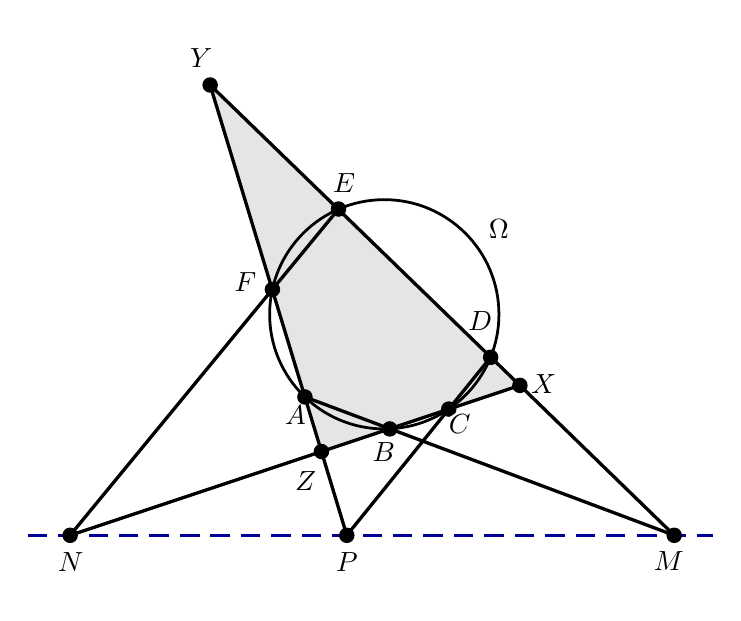
\begin{tikzpicture}[scale = 0.7]
    \clip(-4.89,-1.66) rectangle (7.54,8.6);
    \fill[line width=1.2pt,fill=black,fill opacity=0.1] (-1.58,7.56) -- (0.44,0.91) -- (4.04,2.11) -- cycle;
    \draw [line width=1pt] (1.58,3.4) circle (2.08cm);
    \draw [line width=1pt,dash pattern=on 7pt off 4pt,color=qqqqzz,domain=-4.89:7.54] plot(\x,{(--3.63-0*\x)/-5.94});
    \draw [line width=1.2pt] (-1.58,7.56)-- (0.44,0.91);
    \draw [line width=1.2pt] (0.44,0.91)-- (4.04,2.11);
    \draw [line width=1.2pt] (4.04,2.11)-- (-1.58,7.56);
    \draw [line width=1.2pt] (0.44,0.91)-- (0.9,-0.61);
    \draw [line width=1.2pt] (3.51,2.62)-- (0.9,-0.61);
    \draw [line width=1.2pt] (0.75,5.31)-- (-4.12,-0.61);
    \draw [line width=1.2pt] (0.14,1.9)-- (6.84,-0.61);
    \draw [line width=1.2pt] (4.04,2.11)-- (6.84,-0.61);
    \draw [line width=1.2pt] (0.44,0.91)-- (-4.12,-0.61);
    \draw (3.3,5.3) node[anchor=north west] {$\Omega$};
    \begin{scriptsize}
        \normalsize
        \fill [color=black] (0.14,1.9) circle (4.0pt);
        \draw[color=black] (-0.03,1.57) node[fill = white, rounded corners = 4pt, inner sep=0.4pt] {$A$};
        \fill [color=black] (1.68,1.32) circle (4.0pt);
        \draw[color=black] (1.57,0.9) node[fill = white, rounded corners = 5pt, inner sep=0.8pt] {$B$};
        \fill [color=black] (2.75,1.68) circle (4.0pt);
        \draw[color=black] (2.95,1.41) node[fill = white, rounded corners = 5pt, inner sep=0.8pt] {$C$};
        \fill [color=black] (3.51,2.62) circle (4.0pt);
        \draw[color=black] (3.32,3.27) node[fill = white, rounded corners = 5pt, inner sep=0.8pt] {$D$};
        \fill [color=black] (0.75,5.31) circle (4.0pt);
        \draw[color=black] (0.85,5.78) node[fill = white, rounded corners = 5pt, inner sep=0.8pt] {$E$};
        \fill [color=black] (-0.45,3.85) circle (4.0pt);
        \draw[color=black] (-0.94,3.99) node[fill = white, rounded corners = 5pt, inner sep=0.8pt] {$F$};
        \fill [color=black] (4.04,2.11) circle (4.0pt);
        \draw[color=black] (4.47,2.13) node[fill = white, rounded corners = 5pt, inner sep=0.8pt] {$X$};
        \fill [color=black] (-1.58,7.56) circle (4.0pt);
        \draw[color=black] (-1.74,8.04) node[fill = white, rounded corners = 5pt, inner sep=0.8pt] {$Y$};
        \fill [color=black] (0.44,0.91) circle (4.0pt);
        \draw[color=black] (0.15,0.37) node[fill = white, rounded corners = 5pt, inner sep=0.8pt] {$Z$};
        \fill [color=black] (6.84,-0.61) circle (4.0pt);
        \draw[color=black] (6.74,-1.07) node[fill = white, rounded corners = 5pt, inner sep=0.8pt] {$M$};
        \fill [color=black] (-4.12,-0.61) circle (4.0pt);
        \draw[color=black] (-4.11,-1.1) node[fill = white, rounded corners = 5pt, inner sep=0.8pt] {$N$};
        \fill [color=black] (0.9,-0.61) circle (4.0pt);
        \draw[color=black] (0.9,-1.1) node[fill = white, rounded corners = 5pt, inner sep=0.8pt] {$P$};
    \end{scriptsize}
\end{tikzpicture}